% 4up version
%\documentclass[handout, 12pt, aspectratio=169]{beamer}

\documentclass[12pt,aspectratio=169]{beamer}

\usefonttheme{professionalfonts}

\mode<handout>
{
\usepackage{pgfpages}
\pgfpagesuselayout{4 on 1}[a4paper,landscape]
}

\usepackage[english]{babel}
\usepackage{luatexja}
\usepackage{luatexja-fontspec}


% for display code
%\usepackage{minted}
%\newfontfamily\hasklig{hasklig}[NFSSFamily=haskligFamily]
%\setminted[haskell]{fontfamily=haskligFamily,
%mathescape,
%       numbersep=5pt
%}

% for proof tree
%\usepackage{bcprules}

%\usepackage[T1]{fontenc}

%for lualatex
\usepackage{fontspec}
\setsansfont{CMU Sans Serif}%{Arial}
\setmainfont{CMU Serif}%{Times New Roman}
\setmonofont{CMU Typewriter Text}%{Consolas}

\usepackage{lmodern,amsmath,amssymb,proof}
\usepackage{tikz}
\usetikzlibrary{arrows,positioning,cd}



% color scheme
\definecolor{green}{rgb}{0.0,0.5,0.0}
\definecolor{blue}{rgb}{0.0,0.0,0.7}
\definecolor{red}{rgb}{0.8,0.0,0.0}
\definecolor{lightred}{rgb}{1.0,0.97,0.97}
\definecolor{lightblue}{rgb}{0.95,0.95,1.0}
\definecolor{darkblue}{rgb}{0.3,0.3,0.5}
\definecolor{darkred}{rgb}{0.6,0.0,0.0}
\definecolor{darkorange}{rgb}{0.6,0.2,0.1}
\definecolor{darkgreen}{rgb}{0,0.3,0}
%
\newcommand{\IMAGE}[2]{\pgfdeclareimage[#1]{#2}{#2}\pgfuseimage{#2}}

\setbeamerfont{title}{series=\bfseries,size=\Large}
\setbeamercolor{title}{fg=red}
\setbeamerfont{subtitle}{series=\bfseries,size=\LARGE}
\setbeamercolor{subtitle}{fg=red}
\setbeamerfont{author}{series=\bfseries,size=\large}
\setbeamercolor{author}{fg=blue}
\setbeamerfont{institute}{series=\bfseries,size=\large}
\setbeamercolor{institute}{fg=green}

\setbeamertemplate{blocks}[rounded]
\setbeamerfont{block title}{series=\bfseries,family=\sffamily,size=\small\strut}
\setbeamercolor{block title}{bg=darkblue,fg=white}
\setbeamercolor{block body}{bg=blue!4!white}
\setbeamercolor{block title example}{bg=white,fg=darkgreen}
\setbeamercolor{block body example}{bg=white}
\setbeamercolor{block title alerted}{bg=darkred,fg=white}
\setbeamercolor{block body alerted}{bg=red!4!white}
\setbeamercolor{structure}{fg=darkred}
% no fading effect
\makeatletter
\pgfdeclareverticalshading[lower.bg,upper.bg]{bmb@transition}{200cm}{%
  color(0pt)=(lower.bg); color(4pt)=(lower.bg); color(4pt)=(upper.bg)}
\makeatother

% frametitle
\useframetitletemplate{
\begin{centering}
\centerline{\large\bfseries\color{darkblue}\insertframetitle}
\end{centering}
}

% footer  (title  page/pages)
\setbeamertemplate{navigation symbols}{}
\useheadtemplate{\vbox{\vskip8pt}}
\usefoottemplate{\vbox{\vskip2pt\inserttitle\hfil\insertframenumber/\inserttotalframenumber\vskip5pt}}

% enumerate/itemize environment
\newcommand*\tikzboxed[1]{\tikz[baseline=(c.base)]{%
\node[thick,shape=rectangle,draw,inner sep=2pt] (c) {#1};}}
\setbeamertemplate{items}[square]
\setbeamertemplate{enumerate item}{\tikzboxed{\footnotesize\insertenumlabel}}
\setlength{\itemsep}{1ex}

\newcommand{\m}[1]{\mathsf{#1}}
\newcommand{\mi}[1]{\mathit{#1}}
\newcommand{\md}[1]{\mathtt{\textcolor{blue}{#1}}}
\newcommand{\seq}[2][n]{{#2_1},\dots,{#2_{#1}}}
%
\newcommand{\FF}{\mathcal{F}}
\newcommand{\RR}{\mathcal{R}}
\newcommand{\VV}{\mathcal{V}}
\newcommand{\TT}{\mathcal{T}}
\newcommand{\Var}{\mathcal{V}\m{ar}}
%
\newcommand{\app}{\circ}

\newlength{\mytotalwidth}
\mytotalwidth=\dimexpr\linewidth-5 mm
\newlength{\mycolumnwidth}
\mycolumnwidth=\dimexpr\mytotalwidth-5 mm

\title{ Chapter1.4 }
\author{Wataru Yachi}
\institute{JAIST}
\date{December 21, 2023}

\begin{document}

\maketitle

\newcommand{\MA}{\mathcal{A}}
\newcommand{\AB}{\alpha/\beta}

\begin{frame}[fragile]
    \frametitle{$\alpha/\beta$ Relation}
    \begin{definition}
        let $\MA = \langle A, \{\alpha,\beta\} \rangle$ be ARS
        \begin{itemize}
            \item \alert{$\AB$} $= \beta^*\alpha\beta^*$
            \item $\alpha$ is \alert{relatively terminating} with respect to $\beta$ if $\AB$ is terminating 
        \end{itemize}
    \end{definition}
    \pause
    \begin{example}
    \begin{columns}[totalwidth=\mytotalwidth]
    \begin{column}[t]{0.5\mycolumnwidth}
    \[
            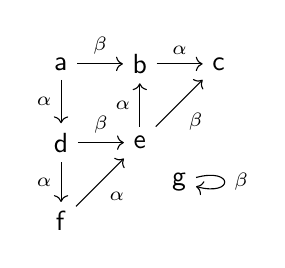
\begin{tikzpicture}[auto]
                \node (a) at (0,0) {$\m{a}$}; \node (b) at (1,0) {$\m{b}$}; \node (c) at (2,0) {$\m{c}$};
                \node (d) at (0,-1) {$\m{d}$}; \node (e) at (1,-1) {$\m{e}$};
                \node (f) at (0,-2) {$\m{f}$}; \node (g) at (1.5, -1.5) {$\m{g}$};

                \draw[->] (a) to node [above]{$\scriptstyle\beta$}(b);
                \draw[->] (b) to node [above]{$\scriptstyle\alpha$} (c);
                \draw[->] (a) to [swap]node{$\scriptstyle \alpha$} (d);
                \draw[->] (d) to [swap]node{$\scriptstyle \alpha$} (f);
                \draw[->] (d) to node{$\scriptstyle \beta$}  (e);
                \draw[->] (f) to [swap]node{$\scriptstyle \alpha$} (e);
                \draw[->] (e) to node{$\scriptstyle \alpha$} (b);
                \draw[->] (e) to [swap]node{$\scriptstyle \beta$}  (c);
                \draw[->,loop right] (g) to node{$\scriptstyle \beta$} (g);
            \end{tikzpicture}
        \]
    \end{column}
        \pause
    \begin{column}[t]{0.5\mycolumnwidth}
            \[
                \alpha/\beta = \alpha \;\cup\; \{
                        (\m{a}, \m{c}), (\m{a},\m{e}), (\m{d},\m{b})\}
            \]
            \pause
            \begin{itemize}
                \item this ARS is not terminating
                \item but $\alpha/\beta$ is terminating
            \end{itemize}
    \end{column}
    \end{columns}
    \end{example}
\end{frame}

\newcommand{\bcab}{\;\beta^* \cup (\alpha/\beta)^*\;}
\newcommand{\bs}{\;\beta^*\;}
\newcommand{\acbs}{\;(\alpha \cup \beta)^* \;}
\newcommand{\asbs}{\;(\alpha/\beta)^*\;}


\begin{frame}
    \begin{lemma}
        $\beta^* \cup (\alpha/\beta)^* \subseteq (\alpha \cup \beta)^*$
    \end{lemma}
    \pause
    \begin{proof}
        We distinguish two cases.
        \pause
        \begin{itemize}
            \item If $a \bs b$ then we have $a\;\beta^* \;b\; (\alpha \cdot \beta^*)^*\;b$.
                \pause
            Since $\beta^* \cdot (\alpha \cdot \beta^*)^* = (\alpha \cup \beta)^*$, $a \acbs b$ holds.
                \pause
            \item If $a \asbs c$ then we perform induction on the length of $\asbs$.
                \begin{itemize}
                    \pause
                    \item If $a = c$ then $a \acbs c$ holds.
                    \pause
                    \item If $a \;\alpha/\beta\; b \; (\alpha/\beta)^* c$ then by I.H., we have $b \acbs c$.
                    \pause
                    Since $a \bs a' \; \alpha \; b' \bs b$, we have $a \acbs a'$, $a' \acbs b'$, and $b' \acbs b$.
                    \pause
                    Hence $a \acbs c$ holds.
                \end{itemize}
        \end{itemize}
    \end{proof}
\end{frame}

\begin{frame}
    \begin{lemma}
        $(\alpha \cup \beta)^* \subseteq \beta^* \cup (\alpha/\beta)^*$
    \end{lemma}
    \pause
    \begin{proof}
        We show that $(\alpha \cup \beta)^n \subseteq \beta^* \cup (\alpha/\beta)^*$ for all $n \in \mathbb{N}$ by induction on $n$.
        \pause
        \begin{itemize}
            \item If $n = 0$ and $a\; (\alpha \cup \beta)^n \; b$ then $a =b$. So $a \bs b$.
            Hence the claim holds.
            \pause
            \item If $n > 0$ and $a\; (\alpha \cup \beta)^{n-1} \; b \; \alpha \cup \beta\; c$
            then we have $a \;\beta^* \cup (\alpha/\beta)^*\; b$ by I.H. So we have four cases.
            \pause
            \begin{itemize}
                \item If $a \bs b$ and $b\; \alpha \;c$ then $a\; \alpha/\beta\;c$. So $a\; \beta^* \cup (\alpha/\beta)^*\; c$ holds.
                \pause
                \item If $a \bs b$ and $b \;\beta\; c$ then we have $a \bs c$. So $a\; \beta^* \cup (\alpha/\beta)^*\; c$ holds.
                \pause
                \item If $a \; (\alpha/\beta)^*\; b$ and $b \; \alpha \;c$ then
                \pause
                since $b\; \alpha/\beta\; c$, we have $a \; (\alpha/\beta)^*\; c$. So the claim holds.
                \item If $a \; (\alpha/\beta)^*\; b$ and $b \; \beta \; c$ then we distinguish two cases.
                \pause
                If $a = b$ then $a \bs c$. So the claim holds.
                \pause
                If $a \;(\alpha/\beta)^* \cdot \alpha/\beta\; b$ then we have $a \;(\alpha/\beta)^*\;$.
                Hence the claim holds. 
            \end{itemize}
        \end{itemize}
    \end{proof}
\end{frame}

\begin{frame}
    \begin{lemma}
        $\beta^* \cup (\alpha/\beta)^* = (\alpha \cup \beta)^*$
    \end{lemma}
    \pause
    \begin{proof}
        By previous lemmata, we have
        $\beta^* \cup (\alpha/\beta)^* \subseteq (\alpha \cup \beta)^*$ and
        $(\alpha \cup \beta)^* \subseteq \beta^* \cup (\alpha/\beta)^*$.
        So $\beta^* \cup (\alpha/\beta)^* = (\alpha \cup \beta)^*$ holds.
    \end{proof}
\end{frame}

\begin{frame}
\begin{lemma}
    for all ARS $\MA = \langle A, \{\alpha,\beta\} \rangle$, following statements are equivalent
    \begin{enumerate}
        \item $\alpha$ is relatively terminating with respect to $\beta$
        \item $\beta^*\alpha$ is terminating
        \item $\alpha\beta^*$ is terminating
    \end{enumerate}
\end{lemma}
    \pause
\begin{proof}
    Exercise 1.34 (a) 
\end{proof}

\end{frame}
\newcommand{\bto}{\to_{\beta}}
\newcommand{\ato}{\to_{\alpha}}

\begin{frame}
    \frametitle{Termination from Relative Termination}
    \begin{lemma}
        %let $\MA = \langle A, \{\alpha,\beta\} \rangle$ be ARS\\
        if $\AB$ and $\beta$ are terminating then $\MA$ is terminating
    \end{lemma}
    \pause
    \begin{proof}
        Suppose $a_0 \to a_1 \to a_2 \to \cdots$.
        \pause Since $\alpha$ is relatively terminating
        with respect to $\beta$, the sequence contains only finitely many $\ato$.
        \pause
        So there exists some $i \in \mathbb{N}$ such that
        $a_i \bto a_{i+1} \bto a_{i+2} \bto \cdots$. 
        pause
        However $\beta$ is terminating.
        \pause
        So $a_i \bto a_{i+1} \bto a_{i+2} \bto \cdots$ is terminating.
        \pause
        Hence we have contradiction.
    \end{proof}
\end{frame}

\begin{frame}[fragile]
    \frametitle{Quasi-commutation}
    \begin{definition}
        %let $\MA = \langle A, \{\alpha,\beta\} \rangle$ be ARS\\
        $\alpha$ \alert{quasi-commutes} over $\beta$ if
        \begin{tikzcd}
            \cdot & \cdot \\
            \cdot & \cdot
            \arrow["\beta", from=1-1, to=1-2]
            \arrow["\alpha", from=1-2, to=2-2]
            \arrow["\alpha"', dashed, from=1-1, to=2-1]
            \arrow["{*}", dashed, from=2-1, to=2-2]
        \end{tikzcd}
    \end{definition}
    \pause

    \begin{example}
        \centering
            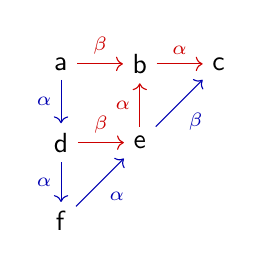
\begin{tikzpicture}[auto]
                \node (a) at (0,0) {$\m{a}$}; \node (b) at (1,0) {$\m{b}$}; \node (c) at (2,0) {$\m{c}$};
                \node (d) at (0,-1) {$\m{d}$}; \node (e) at (1,-1) {$\m{e}$};
                \node (f) at (0,-2) {$\m{f}$};

                \draw[->, red] (a) to node [above]{$\scriptstyle\beta$}(b);
                \draw[->, red] (b) to node [above]{$\scriptstyle\alpha$} (c);
                \draw[->, blue] (a) to [swap]node{$\scriptstyle \alpha$} (d);
                \draw[->, blue] (d) to [swap]node{$\scriptstyle \alpha$} (f);
                \draw[->, red] (d) to node{$\scriptstyle \beta$}  (e);
                \draw[->, blue] (f) to [swap]node{$\scriptstyle \alpha$} (e);
                \draw[->,red] (e) to node{$\scriptstyle \alpha$} (b);
                \draw[->, blue] (e) to [swap]node{$\scriptstyle \beta$}  (c); 
            \end{tikzpicture}
        \pause
        $\alpha$ quasi-commutes over $\beta$
    \end{example}
\end{frame}



\begin{frame}[fragile]
    \begin{lemma}
        if $\alpha$ quasi-commutes over $\beta$ then $\alpha$ quasi-commutes over $\beta^*$
    \end{lemma}
    \pause

    \begin{proof}
        We show that for all $n \in \mathbb{N}$,
        $\alpha$ quasi-commutes over $\beta^n$ by induction on $n$.
        \pause
        \begin{columns}[totalwidth=\mytotalwidth]
            \begin{column}[t]{0.5\mycolumnwidth}
            If $n = 0$ then
            \[
                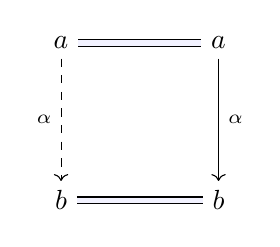
\begin{tikzpicture}[auto]
                    \node (a) at (0,0) {$a$}; \node (b) at (2,0) {$a$};
                    \node (d) at (0,-2) {$b$}; \node (e) at (2,-2) {$b$};
                    \draw [double distance=2pt,double=lightblue](a) to (b);
                    \draw[->] (b) to node{$\scriptstyle \alpha$}(e);
                    \draw[->,dashed] (a) to [swap]node{$\scriptstyle \alpha$}(d);
                    \draw [double distance=2pt,double=lightblue](d) to (e);
                \end{tikzpicture}
                \]
            \end{column}
            \pause
            \begin{column}[T]{0.5\mycolumnwidth}
            If $n > 0$ then
            \[
            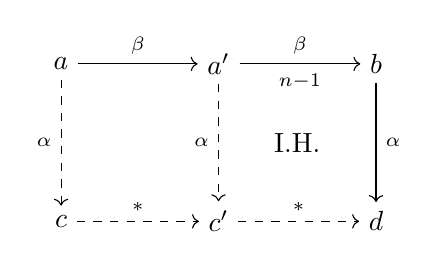
\begin{tikzpicture}[auto]
                \node (a) at (0,0) {$a$}; \node (b) at (2,0) {$a'$}; \node (c) at (4,0) {$b$};
                \node (d) at (0,-2) {$c$}; \node (e) at (2,-2) {$c'$}; \node (f) at (4,-2) {$d$};
                \node (i) at (3,-1) {I.H.};
                \draw[->] (a) to node [above]{$\scriptstyle\beta$}(b);
                \draw[->] (b) to node {$\scriptstyle\beta$} (c);
                \draw[] (b) to node [below]{$\scriptstyle n-1$} (c);
                \draw[->] (c) to node{$\scriptstyle \alpha$} (f);
                \draw[->, dashed] (e) to node{$\scriptstyle *$} (f);
                \draw[->, dashed] (d) to node{$\scriptstyle *$} (e);
                \draw[->, dashed] (b) to [swap]node{$\scriptstyle \alpha$}(e);
                \draw[->, dashed] (a) to [swap]node{$\scriptstyle \alpha$}(d);
            \end{tikzpicture}
            \]
        \end{column}
    \end{columns} 
    \end{proof}
\end{frame}

\newcommand{\abto}{\to_{\alpha/\beta}}

\begin{frame}
    \frametitle{}
    \begin{lemma}
        if $\alpha$ quasi-commutes over $\beta$,
        every $\alpha$-terminating element $a$ is $\alpha/\beta$-terminating
    \end{lemma}
    \pause
    \begin{proof}
        Let $a$ be an $\alpha$-terminating element.
        \pause
        We perform well-founded induction on $a$.
        \pause
        %We distinguish two cases.
        \begin{itemize}
            \item If $a \in \mathsf{NF}(\alpha/\beta)$, the claim is trivial.
            \pause
            \item If $a \abto b$, by the quasi-commutation of $\alpha$ over $\beta^*$, we have
            $a \ato a' \to^* b$.
            \pause Since $a$ is $\alpha$-terminating and $a \ato a'$,
            $a'$ is $\alpha$-terminating.
            \pause By I.H., $a'$ is $\alpha/\beta$-terminating.
            \pause
            Because $(\alpha \cup \beta)^* = \beta^* \cup (\alpha/\beta)^*$,
            we observe two cases.
            \begin{itemize}
                \pause
                \item If $a' \abto^* b$, trivially $b$ is $\alpha/\beta$-terminating.
                \pause
                \item If $a' \bto^* b$, since $\alpha/\beta$-termination is preserved under $\bto^*$,
                    $b$ is $\alpha/\beta$-terminating. 
            \end{itemize}
        \end{itemize}
    \end{proof}

\end{frame}

\begin{frame}
    \begin{corollary}
        let $\MA = \langle A, \{\alpha,\beta\} \rangle$ be an ARS such that $\alpha$ quasi-commutes over $\beta$\\
        if $\alpha$ and $\beta$ is terminating then $\mathcal{A}$ is terminating
    \end{corollary}
\end{frame}

\end{document}
